%=========================================
% 	   Grundlagen     		 =
%=========================================
\chapter{Grundlagen}
\label{ch:grundlagen}
Um die Cloud Native Architektur zu betrachten, gilt es erst einige Grundlagen zu erarbeiten. In diesem Kapitel wird zunächst der Begriff Cloud abgegrenzt. Dabei wird auch der unterschied von \textit{Public} und \textit{Private Cloud} betrachtet. Daraus wird anschließend eine Liste von Anforderungen an eine Cloud-Architektur formuliert. Aufbauend auf dieser wird abschließend die Cloud Native Architektur definiert und deren Eigenschaften betrachtet. 

\section{Die Cloud}
Der Begriff Cloud ist heutzutage sowohl in Fachliteratur, als auch in it-fernen Bereichen vorzufinden. Dabei wird der Begriff \textit{Cloud} als Oberbegriff für neue Technologien und Produkte verwendet.\\ 
Dafür gilt es zunächst zu ermitteln, in welcher Umgebung Cloud-Applikationen betrieben werden.\\\\
Die NIST definiert \textit{Cloud Computing}, als ein Model für allgegenwärtigen Zugriff auf eine geteilte Menge von Rechenleistung. Diese kann durch ein Service-Provider schnell bereitgestellt oder freigegeben werden. Der Kunde kann demnach flexibel Rechenleistung dazu kaufen, oder die bereitgestellte Rechenleistung verringern. Hierfür ist keine menschliche Kommunikation von Nöten. Deshalb wird dies von der NIST als \textit{On-demand self-service} bezeichnet.\\
Um dies zu ermöglichen nutzt der Service-Provider das sogenannte \textit{Resource-Pooling}. Hierfür teilt der Service-Provider dem Kunden automatisiert Rechenleistung zu. Der Kunde hat hierbei nur begrenzt Einfluss auf den Standort oder die genaue Maschine, welche die Leistung zur Verfügung stellt.\cite{mell_nist_2011}\\
Der Kunde bezahlt folglich Rechenleistung, und nicht einzelne Maschinen. Die Cloud kann demnach als Pradigma für das Hosten und Bereitstellen von Services über das Internet gesehen werden \cite{avram_advantages_2014}.

\subsection{Service Modelle}
Verschiedene Geschäftsmodelle des Cloud-Computings setzen unterschiedliche Grade der Abstraktion um. Hierbei wird zwischen den Service Modellen \textit{Infrastructure as a Service}, \textit{Plattform as a Service} und \textit{Software as a Service} unterschieden. Im Nachfolgenden werden diese Modelle voneinander abgegrenzt.
\subsubsection{Infrastructure as a Service}
Das sogenannte\textit{ Infrastructure as a Service (IaaS)}\cite{mell_nist_2011} stellt Speicher -und Rechenleistung zur Verfügung. Der Kunde muss also nicht selbst physische Hardware betreiben. IaaS kann als Grundschicht unter allen anderen Service Modellen gesehen werden.\\
Mittels Virtualisierung teilt der Service-Provider die physische Hardware auf und teilt sie den Kunden zu. Der  Kunde hat also kein Einfluss auf die zugrundeliegende Infrastruktur. Allerdings kann er Aspekte wie Speicher, Betriebssystem, Middle-Ware und die Anwendung selbst konfigurieren \cite{dimpi_rani_rajiv_kumar_ranjan_comparative_2014}.\\
Auch ein begrenzter Zugriff auf Netzwerkomponenten, wie zum Beispiel die Firewall, kann möglich sein. IaaS stellt demnach die selben Funktionen wie ein traditionelles  Rechen-Center zur Verfügung. Der Kunde muss allerdings kein solches Instandhalten und kann flexibel die Rechenleistung erhöhen oder verringern. \\
Abgerechnet wird in der Regel entsprechend der Nutzungsdauer. In einigen Fällen übernimmt der Service-Provider auch Aufgaben wie die Systemwartung, Datensicherung und das Notfall-Management.\\
Unter anderem sind Microsoft, IBM und Amazon Anbieter von IaaS Angeboten. \cite{simon_lohmann_iaas_nodate} \cite{mell_nist_2011}
\subsubsection{Plattform as a Service}
Das \textit{Plattform as a Service (PaaS)}\cite{mell_nist_2011} Model abstrahiert gegenüber IaaS weitere Aspekte der Cloud. Weiterhin muss der Kunde keine eigene Rechenzentren verwalten und erhält durch den Service Provider flexibel Rechenleistung.\\
Allerdings werden nun auch Aspekte wie das Betriebssystem, die Speicherverwaltung mit Datenbanken und das Netzwerk, durch den Service Provider verwaltet. Der Kunde erhält eine Entwicklungsumgebung in der Cloud, über welche der die Anwendung bereitstellen kann. \\
PaaS ist dafür konzipiert den kompletten Lebenszyklus einer Anwendung zu ermöglichen. Hierzu zählen das bauen, testen, veröffentlichen, verwalten und aktualisieren einer Anwendung \cite{dimpi_rani_rajiv_kumar_ranjan_comparative_2014}. Auf einer höheren Abstraktion kommen neben Entwicklungswerkzeugen, Programmiersprachen, Bibliotheken und Datenbanken auch Container-Techniken dazu.\\
Zu den wichtigsten PaaS Anbietern gehören Amazon, IBM und Microsoft. \cite{simon_lohmann_platform_nodate}\cite{sowmya_layers_2014} \cite{mell_nist_2011} 
\subsubsection{Software as a Service}
\textit{Software as a Service (SaaS)} ist die am meisten abstrahierte Form des Cloud-Computings. Kunden können über das Internet auf Angebote zugreifen, welche von einem Service-Provider zur Verfügung gestellt werden. Die Applikation wird durch den Service-Provider verwaltet, betrieben und aktualisiert. \\
Der Nutzer verwaltet keinen Aspekte der zugrundeliegenden Infrastruktur. Einzig eine konfigurieren der Anwendung selbst kann möglich sein.\\
Typische SaaS-Applikationen im Business Bereich sind \textit{Google G Suite} \cite{noauthor_google_nodate}  und \textit{Microsoft Office 365} \cite{noauthor_office_nodate}. \\
SaaS-Provider rechnen Anwendungen in der Regen anhand bestimmter Parameter, wie die Anzahl der Nutzer, ab. Auch bei SaaS-Angeboten können Kunden bei Bedarf einzelne Dienste oder Funktionen stärker in Anspruch nehmen. \cite{wolfgang_herrmann_saas_nodate} \cite{sowmya_layers_2014} \cite{mell_nist_2011}

\subsection{Deployment Modelle}
Neben dem Grad der Abstraktion stellt auch der Ort der Hardware eine Rolle. Wird diese lokal von dem eigenen Unternehmen verwaltet? Oder ist eine externe Firma dafür verantwortlich? Hierfür existieren einige Modell, welche im Folgenden voneinander differenziert werden:
\begin{description}
    \item [on premise] \hfill \\ Auch als on-premise Cloud oder private Cloud bezeichnet \cite{dimpi_rani_rajiv_kumar_ranjan_comparative_2014}. Die Infrastruktur wird exklusiv von einer Organisation genutzt \cite{mell_nist_2011}. Die Verwaltung der Infrastruktur kann ebenfalls durch diese Organisation erfolgen. Alternativ kann eine externe Firma damit beauftragt werden. Die benötigte Hardware befindet sich entweder in-house (\textit{on-premise}) oder oder wird \textit{off-premise} extern bereitgestellt \cite{zwicker_saas_nodate}.
    \item [public Cloud] \hfill \\ Die Infrastruktur wird durch einen Dritt-Anbieter über das Internet zur Verfügung gestellt. Die gesamte Hardware ist im Besitzt des Service-Providers. Die selbe Hardware, Speicher und Netzwerk-Geräte des Service-Providers werden mit anderen Kunden geteilt. Beispiele hierfür wären Microsoft Azure oder Amazon Web Services. \cite{microsoft_public_nodate} \cite{mell_nist_2011}
    \item [hybrid Cloud] \hfill \\ Hybrid Clouds bestehen aus mehreren getrennten Cloud-Infrastrukturen. Daten und Applikationen einer hybrid Cloud können zwischen private Cloud und public Cloud Infrastrukturen wechseln. \cite{mell_nist_2011}
\end{description}

\subsection{Vorteile und Möglichkeiten der Cloud}
Jedes der oben genannten Deployment Modelle und Service Modelle hat eine Menge von Eigenschaften gemeinsam. Avram et al. nennt folgende Eigenschaften: (i) pay-per-use (kein vortlaufenden Verpflichtungen), (ii) elastic capacity and the illusion of infinite resources; (iii) self-service-interface; und (iv) resources that are abstracted or virtualized \cite{avram_advantages_2014}. Aus diesen folgend direkt einige Vorteile des Cloud-Computings.
\begin{itemize}
  \item Durch das pay-per-use Modell muss der Kunde nur für die Leistung zahlen, die er tatsächlich benötigt. Dies reduziert Hardware-Kosten, wie auch die Kosten für Verwaltung, Software-Updates und den Strom. Ferner wird weniger Personal für die Verwaltung der IT benötigt. Dies ermöglicht auch kleineren Firmen rechen-aufwändige Analysen zu bewältigen. Letztere waren zuvor nur größeren Firmen vorbehalten. Diese umfangreichen Berechnungen benötigen meist viel Leistung, für einen kurzen Zeitraum. Durch das self-service-interface (iii) und die dynamische Kapazität von Leistung (iv) mit pay-per-use (i) ist dies möglich. Avram et al \cite{avram_advantages_2014} sieht hier zusätzlich eine Möglichkeit für Dritte-Welt-Länder zu dem Westen aufzuschließen. Länder welche traditionell nicht die benötigen Ressourcen gehabt hätten, können nun diese durch Cloud-Computing beziehen.  
  \item Durch das Cloud-Computing können neue Business-Modell umgesetzt werden. Die Cloud ermöglicht einen direkten Zugriff auf Rechenleistung, ohne eine Vorherige Kapital-Anlage des Kunden \cite{noauthor_premise_2020}. Es muss nicht zuvor Geld in ein Rechenzentrum oder zusätzliche IT-Experten investiert werden. Die Zeit bis ein neues Produkt gewinnbringend an den Markt gebracht werden kann, ist demnach deutlich gesunken. Viele Internet-Startups konnten dadurch gegründet und zum Erfolg geführt werden \cite{avram_advantages_2014}. 
  \item Cloud-Computing erleichtert des Firmen, ihre Services zu skalieren. Wächst die Zahl der Nutzer, kann Rechenleistung dazu gekauft werden. Die Kosten steigen daher dynamisch mit der Reichweite des Unternehmens. Auch eine Reaktion auf ein kurzfristigen Anstieg oder Abfall der Nutzer-Anfragen ist möglich. Eines der Ziele des Cloud-Computings besteht darin, Ressourcen mithilfe von Software-APIs je nach Client-Auslastung bei minimaler Interaktion mit dem Service-Provider dynamisch zu vergrößern oder zu verkleinern \cite{avram_advantages_2014}. Dies ist möglich, da die Rechen-Ressourcen durch Software verwaltet werden. Für eine dynamische Skalierung, wird zusätzlich eine passende Software-Architektur benötigt. Hierauf wird in einem späteren Kapitel eingegangen.
  \item Hier ist außerdem der Gedanke aufzugreifen, dass eine Fokussierung auf das Geschäftsmodell möglich wird. Firmen können sich auf ihr eigentliches Geschäftsmodell konzentrieren. Zeit und Geld können in das Geschäftsmodell und nicht in die IT-Infrastruktur investiert werden.
\end{itemize}

\section{Anforderungen}\label{grundlagen_anforderungen}
Nachdem wir im letzten Abschnitt den Begriff Cloud-Computing erläutert haben, gilt es nun Cloud-Applikationen zu betrachten. Die meisten der zuvor genannten Vorteile des Cloud-Computings können nur durch eine passende Software-Architektur vollkommen ausgeschöpft werden. Beim Entwurf der Architektur einer Cloud-Applikation müssen einige Aspekte beachtet werden. Folgende Anforderungen haben sich dabei herauskristallisiert:
\begin{itemize}
    \item Cloud-Applikationen operieren meist global. Dies heißt nicht nur, dass der Dienst stets über das Internet erreichbar ist. Bei der Betrachtung von globalem Zugriff muss berücksichtigt werden, dass der Dienst in lokalen Rechenzentren dupliziert werden muss \cite{gannon_cloud-native_2017}. Nur so kann eine geringe Latenz garantiert werden. Dabei führt die Integrität von Daten häufig zu Problem. Diese müssen stets dem Nutzer zur Verfügung stehen. Dem Nutzer darf nicht ersichtlich sein, dass seine Daten an mehreren Orten abgespeichert sind.  
    \item Cloud-Applikationen müssen mit vielen tausend von parallelen Nutzern operieren können. Neben einer vertikalen Skalierung (mehr und bessere Hardware) wird demnach auch eine horizontale Skalierung nötig \cite{gannon_cloud-native_2017}. Diese wird meist durch Parallelisierung umgesetzt. Eine horizontale Skalierung führt erneut zu einem Fokus auf die Konsistenz und Synchronisation des Systems. 
    \item Die Architektur einer Cloud-Applikationen muss mit der Annahme entwickelt werden, dass die Hardware nicht konstant ist und Fehler vorkommen werden. Gannon et Al. \cite{gannon_cloud-native_2017} sieht Probleme bei Applikationen, welche nicht für die Cloud entwickelt wurden. Diese nehmen an, dass die Hardware und das Betriebssystem konstant sind. Der kleinste Fehler im Rechenzentrum oder des Netzwerks führt hier bereits zu Fehlern. 
    \item Cloud-Applikationen müssen die Anforderungen an Verteilte-Systeme beachten \cite{scholl_cloud_2019}. Als Beispiel soll das sogenannte CAP-Theorem erwähnt werden \cite{julianbrowne_brewers_nodate}. Ohne eine Optimierung für den Ausfall einzelner (Teil-)Systeme ist die Anforderung \textit{Partition Tolerance} des CAP-Theorem nicht erfüllt. Es stellt sich also heraus, dass verteilte Systeme eine Reihe von Anforderungen mit sich bringen. Die Architektur muss demnach damit umgehen, dass sich Dienste nicht auf der selben Maschine befinden. Es wird folglich mit einem Netzwerk von Maschinen gearbeitet. Es wird die Welt der Verteilten Systeme betreten. Diese bringt eine Reihe von eigenen Anforderungen mit sich. Oft werden hier Falsch-Annahmen gemacht. Scholl et Al. \cite{scholl_cloud_2019} nennt diese Annahmen "Fallacies of Distributed Systems". Dazu gehören Aussagen wie unter Anderem "the Network is reliable", "Latency is zero" oder "There is infinite bandwith". All diese Aspekte führen zu eigenen Anforderungen, welche die Architektur beachten muss.
    \item Die meisten Cloud-Applikationen werden für den Dauerbetrieb entwickelt. Ein zugriff der Nutzer soll stets möglich sein. Hier ist außerdem der Gedanke aufzugreifen, dass Firmen  Verträge mit dem Kunden haben können. Diese beschränken eine mögliche Downtime auf wenige Stunden im Jahr. Ein Einspielen von Updates darf demzufolge nicht zu einer Downtime für den Nutzer führen. Zudem müssen diese Updates stets getestet werden. Auch Fehler im System oder Abstürze einzelner Knoten dürfen nicht das gesamte System, oder einzelne Funktionen dessen, lahmlegen. Ein umfangreiche Überwachung des Systems und das vorhalten von Ersatzkonten sind nur einige der wichtigen Operationen.\cite{gannon_cloud-native_2017}
\end{itemize}
Zusammenfassend lässt sich sagen, dass Entwickler und Software-Architekten drei großen Herausforderungen der Cloud gegenüber stehen. Zunächst müssen sie verteilte Systeme verstehen. Eine Anforderungen, welche so vorher schon relevant war, allerdings nun noch prominenter in den Vordergrund dritt. Ferner müssen sich Entwickler mit neuen Technologien wie Containern vertraut machen. Und abschließend müssen sie sich bewusst werden, welche Patterns in der Cloud funktionieren.

\section{Prinzipien einer Cloud Native Architektur}
Nachdem nun die Begriffe Cloud-Computing und Cloud-Applikationen beleuchtet wurde, kann eine Architektur für die Cloud betrachtet werden. Das Ziel dieser ist, die Möglichkeiten der Cloud maximal zu Nutzen. Traditionelle Infrastrukturen (on-premise Service Modelle) fokussieren sich auf eine feste Anzahl an Hardware-Komponenten und deren Leistung. Der Cloud-Service-Provider teilt die Leistung allerdings flexibel zu. Folglich nutzen Cloud-Native Architekturen Prinzipien, wie das horizontale Skalieren und automatische Ersetzen von abgestürzten Komponenten um Leistung und Elastizität bereit zu stellen.\\
Sowohl Scholl et Al.\cite{scholl_cloud_2019} , als auch Microsoft, Amazon und Google \cite{tom_grey_5_nodate} definieren eine Vielzahl von Eigenschaften einer Cloud-Native Architektur. Im Folgenden werden diese Eigenschaften beleuchtet. 
\subsection{Automatisierung}
Eines der Ziele einer Cloud-Native Architektur ist es, so viele Aspekte des Systems wie möglich zu automatisieren. Scholl et Al.\cite{scholl_cloud_2019} bezeichnet diese Eigenschaft als ''Operational Excellence''. Ganz natürlich kommt hier das Continuous Integration / Continuous Delivery (CI/CD) ins Spiel. CI/CD beschreibt das automatisierte bauen, testen und deployen des Systems. Auch das Zurücksetzen von Updates (\textit{Rollback}) sollte automatisiert werden.\\
Neben diesen Apsekten ist auch das Logging zentral. \\
Eine Überwachung der Anwendung sollte ebenfalls Implementiert werden. Diese führt dazu, dass Fehler frühzeitig erkannt werden können. Darüber hinaus hat diese auch weitere Vorteile.\\
Aspekte der Cloud wie das on-demmand-self-service ermöglichen es, im Code der Anwendung selbst, die Umgebung der Anwendung anzupassen. So kann ein System sich selbst neue Ressourcen buchen und anwenden. Ein Beispiel wäre hier die Speicherplatzüberwachung. Ist eine Speichereinheit ausgelastet, müsste ein on-premise Deployment Modell auf physische Hardware-Erweiterung warten. Durch das Cloud-Computing kann nun die Software selbst neue Ressourcen buchen. Dies ist führt zu weniger Down-Time und reduziert die Aufgabe von Personal. Grund-Voraussetzung dafür ist eine planvolle Automatisierung und Überwachung.\\ 
Hinzu kommt außerdem, dass eine Cloud-Native-Applikation ein verteiltes System ist. Dadurch ergeben sich neue Fehler-Quellen. Diese sind oft schwer zu testen. Eine Cloud-Native Architektur sollte auch auf diese automatisiert reagieren.\\
Weiterhin lässt sich das Skalieren des Systems automatisieren. Durch das herauf Skalieren bleibt das System weiter erreichbar, und durch das herunter Skalieren werden die Kosten reduziert.\\
Scholl et Al.\cite{scholl_cloud_2019} nennt zudem die Anforderung "Document everything". Eine Automatisierung und Überwachung können nur dann sinnvoll und funktional sein, wenn diese auch klar dokumentiert sind. Jedes Team-Mitglied muss bewusst sein, wie die Umgebung der Anwendung definiert ist und wie die Anwendung auf Ereignisse automatisiert reagiert. Ebenso wie die Anwendung selbst, lässt sich auch das Dokumentieren, mit geeigneten Tools, automatisieren.
\subsection{Sicherheit}
Typisch für Cloud Native Architekturen ist der \textit{defense-in-depth} Sicherheits-Ansatz. Hierbei ist nicht eine zentrale Instanz für die Sicherheit des Systems zuständig. Jede Kommunikation zwischen einzelnen Komponenten des Systems ist abgesichert. Dies schließt eine sichere Verbindung zu dem Source-Code-Repository mit ein. Jede einzelne Komponente, auch wenn diese intern ist, sollte kein Grund-Vertrauen zu anderen Komponenten des Systems haben. Jede Komponente sollte sich vor den anderen Schützen.
\subsection{Sinnvoller Einsatz von State}
Die Speicherung von \textit{State} beschreibt zum einen die Speicherung von Nutzerdaten (z.B. die Einträge in dem Warenkorb des Nutzers) und den Status des Systems (z.B. welche Version des Source-Codes wird gerade im Produktiv-System genutzt). Google beschreibt den State als den schwersten Aspekt von verteilten Systemen \cite{tom_grey_5_nodate}. Daher gilt es nur jene Komponenten des Systems mit State zu füllen, welche diesen tatsächlich benötigen. Komponenten ohne State können erstens einfacher skaliert werden. Zweitens ist bei fehlgeschlagenen Instanzen kein State verloren gegangen. Abschließend ist ein Roll-Back zu einer früheren Version mit \textit{stateless} Komponenten problemloser. Auch hier muss kein inkompatibler State vermieden werden. 

\section{Cloud-Native Technologien}
Die Umsetzung einer Cloud-Native Architektur kann mit \textit{Cloud-Native Technologien} gelöst werden.\\
Die \textit{Cloud Native Computing Foundation} (CNCF) wurde 2015 durch die Linux Foundation gegründet \cite{cncf_new_2015}. Weitere Gründungsmitglieder waren unter anderem Google, RedHat, Huawei und Twitter \cite{}. Neben Beispiel-Projekten, einer Liste von Cloud-Native Technologien und weiteren Ressourcen definiert die CNCF auch Cloud-Native-Technologien. Diese ''[...] ermöglichen es Unternehmen, skalierbare Anwendungen in modernen, dynamischen Umgebungen zu implementieren und zu betreiben.''\cite{cloud_native_computing_foundation_cncftoc_nodate} Als moderne Umgebungen sind Deployment-Modelle wie die private Cloud, public Cloud und hybrid Cloud zu verstehen. Als Best-Practices sieht die CNCF unter anderem \textit{Micro-Services}, \textit{Container} und \textit{Services-Meshes}, auf welche im Folgenden eingegangen werden soll.

\subsection{Micro-Service Architecture}
Die Grund-Idee dieser Architektur ist es, ein System aus vielen kleinen Bausteinen zu erstellen. Diese Bausteine werden\textit{ Micro-Services} genannt. Sie arbeiten zusammen um die gesamte Funktionalität des Systems zu realisieren. Jeder Micro-Service setzt dabei genau eine Funktionalität um. Ferner hat jeder Micro-Service eine klar-definierte Grenze und API-Schnittstellen. Als Schnittstelle kann zum Beispiel eine REST-Api gewählt werden. \cite{chris_richardson_microservices_nodate}
\begin{figure}[bth] 
  \centering
  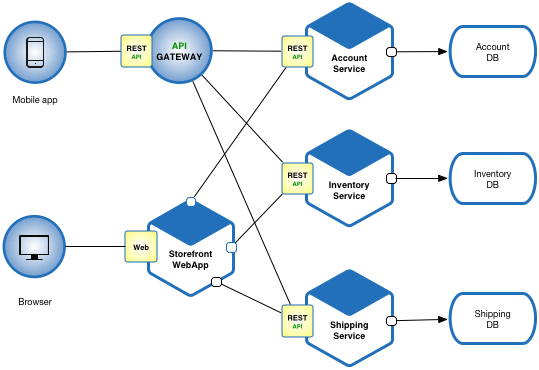
\includegraphics[width=0.7\textwidth]{Chapters/2-Grundlagen/Graphics/Microservice_Architecture.png}
  \caption{Beispielhafter Aufbau einer Micro-Service Architektur \cite{chris_richardson_microservices_nodate}}
  \label{fig:microservices}
\end{figure}
Typischerweise betreut und entwickelt ein Team jeweils einen Micro-Service. \\
Jeder dieser Micro-Services ist einfacher zu Entwickeln und zu Verstehen, als das gesamt System. Dies ermöglicht es Teams die eigene Funktionalität in den Vordergrund zu stellen. Da jeder Micro-Service eine klar definierte API nach außen zur Verfügung stellt, kann gegen diese Entwickelt werden. Für \textit{Service A} ist es nicht von Bedeutung, wie \textit{Service B} seine Funktionalität realisiert. Denn die API von \textit{Service B} ist bekannt und gegen diese wird entwickelt. \textit{Service A} kann demnach die Funktionalität von \textit{Service B} nutzen, ohne deren inneren Aufbau zu kennen. Dies führt auch dazu, dass \textit{Service B} schneller Änderungen vornehmen kann. Die API von \textit{Service-B} bleibt konstant. Daher ist \textit{Service-A} von internen Änderung in \textit{Service-B} nicht betroffen. \\
Ferner wird es durch die Aufteilung in Micro-Services möglich einzelne Bausteine des Systems zu skalieren. Dies spart Kosten gegenüber dem Service-Provider. Dazu kommt, dass einzelne Bausteine des Systems schneller zu ersetzen sind, sollten sie unerwartet gestoppt werden. \\
Micro-Services helfen einer Cloud-Native-Architektur demnach die Skalierbarkeit und Ausfall-Sicherheit zu verbessern.\\
Abschließend können, durch die einheitliche API, Micro-Services mit verschiedenen Technologien erstellt werden. Ein sicheres und hoch-performantes Backend könnte in Rust erstellt werden. Ein weiterer Anwendungsfall mit vielen parallelen Abläufen in GO und ein Frontend in JavaScript. Jede dieser Komponente wird als Micro-Service umgesetzt und kann mit den anderen Micro-Services kommunizieren. Voraussetzung hierfür ist, dass eine plattform-unabhängige API-Schnittstelle gewählt wird. Hier bietet sich zum Beispiel REST über HTTP(S) an.\cite{newman_building_2021}\\\\
Als Nachteile der Micro-Service Architektur ergibt sich zunächst eine höhere Komplexität auf dem System-Level. Durch die Reduktion der Komplexität in den einzelnen Komponenten, wird es zunehmen umfangreicher das Zusammenspiel dieser zu planen. Unter anderem muss betrachtet werden, wie mit nicht erreichbaren Micro-Services umgegangen wird. Ferner muss die Kommunikation zwischen den Komponenten abgesichert werden. Hier gilt erneut das Stichwort in-depth Security. Auch die Überwachung des Systems wird anspruchsvoller. \cite{newman_building_2021}

\subsection{Container}
\textit{Container} verpacken eine Software mit all ihren Konfigurationen und Abhängigkeiten, wodurch die Applikation zuverlässig und schnell in unterschiedlichen Umgebungen betrieben werden kann.\\
Es genügt einen Container zu starten. Dabei ist die Ausführung der Software nicht von dem Betriebssystem abhängig, welches den Container startet. \cite{docker_what_nodate}\\\\
Dies eliminiert typische CI/CD Fehlerquellen. In einem CI/CD Prozess wird die Software meist durch unterschiedliche Teams entwickelt und getestet. Dabei können Fehler entstehen, welche einzig durch unterschiedliche Konfiguration der Entwicklung und Test-Systeme bedingt sind. Diese Variable lässt sich mit Containern eliminieren. \cite{scholl_cloud_2019}\\
Das selbe vorgehen wurde zuvor mit Virtuellen Maschinen umgesetzt. Dies führt allerdings zu einigen Nachteilen. Virtuelle Maschinen beanspruchen viel Speicherplatz und starten Langsam. Container beheben dies, indem Konstanten wie der Betriebssystem-Kernel unter den Containern geteilt wird. Infolgedessen wird die Isolation zwischen den Containern reduziert. Die Abbildung \ref{fig:vm-vs-container} grenzt Virtuelle Maschinen von Containern ab. Container verschlechtern durch die fehlende Isolation die Sicherheit gegenüber Virtuellen Maschinen. Die Sicherheit muss demnach an anderer Stelle erneut verbessert werden. Der Anspruch von Containern ist nicht die Sicherheit zu erhöhen. Der Vorteil von Containern besteht darin, dass sie unabhängig von der Infrastruktur immer gleich funktionieren werden. Für eine Cloud-Native-Applikation ist dies von Vorteil. Das schnelle starten von Containern führt dazu, dass fehlerhafte Container schnell ersetzt werden können. Auch das horizontale Skalieren ist dadurch schneller umsetzbar. Darüber hinaus werden Fehler-Quellen durch den Service-Provider reduziert. Denn Abhängigkeiten zu Konfigurationen der durch den Service-Provider zur Verfügung gestellten Hardware wird reduziert.\\
Das Arbeiten mit Containern kann unter anderem durch Docker \cite{docker_what_nodate} realisiert werden. 

\begin{figure}[bth] 
  \centering
  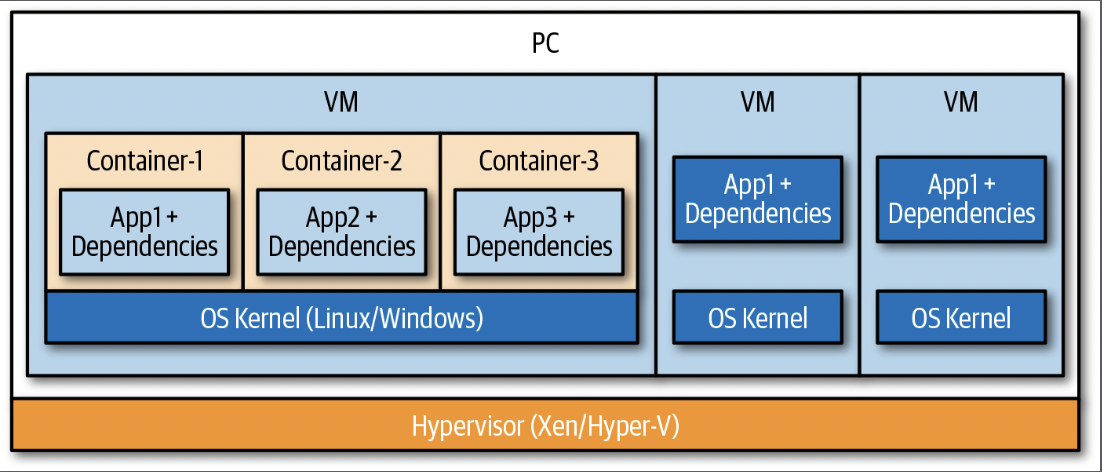
\includegraphics[width=0.7\textwidth]{Chapters/2-Grundlagen/Graphics/container-vs-vm.png}
  \caption{Abgrenzung von Container und Virtueller Maschine \cite{scholl_cloud_2019}}
  \label{fig:vm-vs-container}
\end{figure}

\subsection{Service-Meshes}
Um die Vorteile und Eigenschaften eines Service-Meshes zu betrachten, muss zunächst der Begriff Container-Orchestration beleuchtet werden.
\subsubsection{Container-Orchestration}
Werden die Services einer Micro-Service-Architektur in Containern betrieben, können sie unabhängig von einer festen Infrastruktur betrieben werden.\\
Für eine Cloud-Native Architektur ist dies von Vorteil. Denn Container lassen sich mit minimaler Verzögerung starten und stoppen. Zudem können wir horizontal skalieren, indem wir weitere Container starten. Allerdings ergeben sich dadurch einige Probleme. Zunächst ein Mal müssten Container automatisch gestartet, gestoppt und neu gestartet werden. Die Skalierung des Systems, oder im Fehlerfall das Neu starten von Containern darf keine menschliches Aufgabe sein. Denn dies wäre zwangsläufig mit einer zu großen Verzögerung verbunden.\\
Um diese Verzögerung weiter zu reduzieren, könnten bereits Ersatz-Container vorgehalten werden. Im Fehlerfall oder für die Skalierung würde ein Umleiten des Traffics genügen. Dies erfordert ein automatisiertes Load-Balancing.\\
Ein funktionierendes Load-Balancing ist auch für die Container zu Container Kommunikation notwendig. Wird ein Service durch mehrere Container umgesetzt, gilt es zu definieren, welcher dieser Container adressiert werden soll. Dieses Problem wird als internal Load-Balancing bezeichnet. \\\\

Die\textit{ Container Orchestration}\cite{scholl_cloud_2019} behebt diese Probleme. Der \textit{Container-Orchestrator} liegt als eine Schicht über den Containern. Er ist verantwortlich für das starten und stoppen von Containern. Außerdem teilt er flexibel Rechenleistung zu und skaliert das System passend zum bestehenden Traffic.\\
Stehen mehrere Server zur Verfügung, platziert er neue Container auf den Servern mit der niedrigsten Auslastung. Außerdem verschiebt er Container, sollte die Auslastung zunehmen. Auch andere Metriken sind für die Server Auswahl und die Verschiebung der Container möglich.\\
Der Container-Orchestrator überwacht zudem die Gesundheit der Container. Falls nötig startet er diese neu.\\
Abschließend ist er für das interne und externe Load-Balancing verantwortlich. Realisieren mehrere Container den selben Service, leitet der Load-Balancer den Traffic zu dem geeignetsten Container weiter. \\
Neben den genannten Funktionen kann der Container-Orchestrator auch für das State-Management und viele weitere Aspekte des Systems zuständig sein.\\
Scholl et Al.\cite{scholl_cloud_2019} sieht in Google Kubernetes \cite{kubernetes_production-grade_nodate} die populärste Container Orchestrator Wahl.
\subsubsection{Herausforderungen der Micro-Service-Architektur}
Durch die Aufteilung unserer Anwendung in Micro-Services haben wir die Komplexität der einzelnen Bestandteile unserer Architektur reduziert. Man sollte allerdings bedenken, dass gleichzeitig die Komplexität auf dem System-Level zugenommen hat. Jeder Service einer Micro-Service Architektur wird, neben der Business Logik, unter anderem folgendes enthalten \cite{codingwithnana_istio_nodate}:
\begin{itemize}
    \item Jede Service wird eine Retry-Logik umsetzen. Es ist möglich, dass Services nicht erreichbar sind. Ist dies der Fall, muss definiert werden, wie oft eine Verbindungsversuch unternommen wird. Ferner ist eine Ausnahmebehandlung zu ergänzen.
    \item Darüber hinaus ist die Umsetzung der Sicherheit zu beachten. Eine Firewall kann die Anwendung von außen Schützen. Allerdings gilt es das Konzept der in-depth Security umzusetzen. Diese verlangt, dass auch die Kommunikation unter den Containern abgesichert ist. Ferner sollte nicht jeder Container frei mit jedem anderen Container kommunizieren dürfen.
    \item Abschließend ist für die Automatisierung einer Überwachung unumgänglich. Es gilt Metriken zu erfassen und auf Basis dessen zu Handeln. Logger und Logik zum Fehlerfinden müssen ebenfalls in jedem Service integriert werden.
\end{itemize}
Ein Vorteil der Microservice-Architektur war es, dass jedes Team einen klar getrennten Anteil der Anwendung entwickelt. Allerdings muss jedes Team, neben der eigentlichen Business Logik, die zuvor genannten Funktionen entwickeln, verwalten und konfigurieren. Diese Konfiguration kann nicht individuell für jeden Service statt finden, ohne zu Fehlern und Problem zu führen. Außerdem wird die Fehlersuche deutlich erschwert. Eine Isolation von Fehlern in einem einzigen Service ist nicht mehr sichergestellt.

\subsubsection{Vorgehensweise von Service-Meshes}
\textit{Service Meshes} nutzen einen sogenannten \textit{Sidecar-Proxy} \cite{codingwithnana_istio_nodate}. Dieser wird in Abbildung \ref{fig:service-mesh} dargestellt. Jedem Container wird ein weiterer Container hinzugefügt. Dieser fungiert als Proxy. Er nimmt demnach Verbindungen an und leitet sie zu dem eigentlichen Service weiter. Diese Side-Car-Proxys werden durch die \textit{Control-Plane} verwaltet und in die einzelnen Services injiziert. Ein neuer Service muss demnach die zuvor genannten Probleme, wie Sicherheit oder die Retry-Logic nicht erneut umsetzen. Außerdem ist die Control-Plane eine zentrale Schnittstelle um die gesamte Anwendung zu konfigurieren und zu Überwachen. Neben den genannten Funktionen, kann ein Service-Mesh auch weitere Aspekte, wie zum Beispiel das Load-Balancing, lösen. Meist wird an dieser stelle aber auf einem Container-Orchestrator wie Kubernetes \cite{kubernetes_production-grade_nodate} aufgebaut. Eine mögliches Service-Mesh wäre zum Beispiel Istio \cite{istio_istio_nodate}. 
\begin{figure}[bth] 
  \centering
  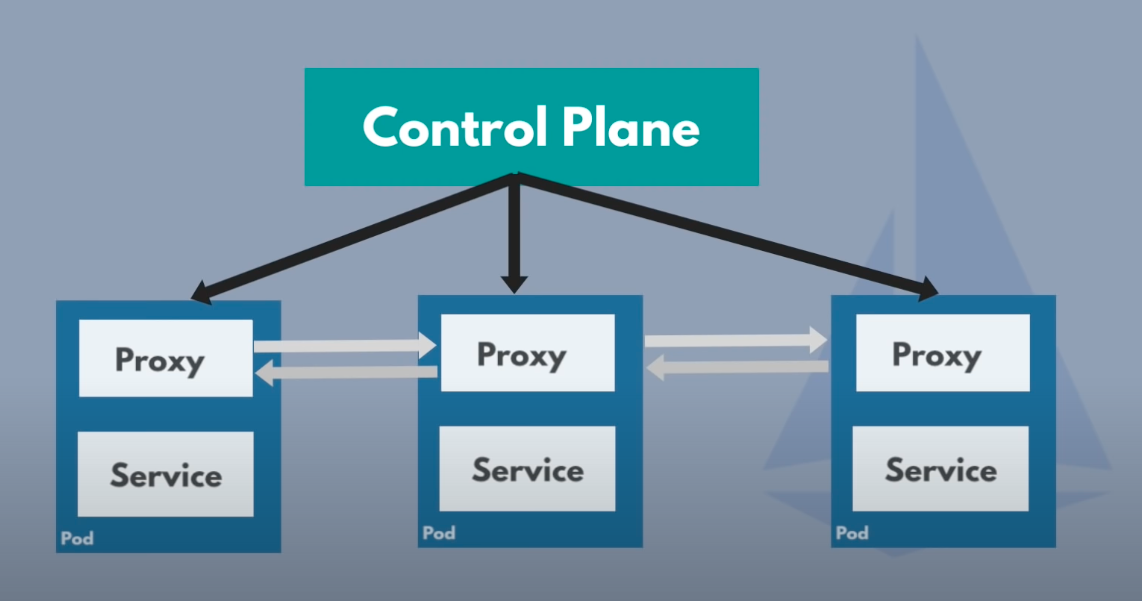
\includegraphics[width=0.7\textwidth]{Chapters/2-Grundlagen/Graphics/service-meshes.png}
  \caption{Service-Meshes am Beispiel Istio \cite{codingwithnana_istio_nodate}}
  \label{fig:service-mesh}
\end{figure}